\documentclass{article}
\usepackage{amsmath}
\usepackage{amsfonts}
\usepackage{amssymb}
\usepackage{graphicx}
\usepackage[parfill]{parskip}
\usepackage{matlab-prettifier}
\usepackage{listings}
\usepackage{xcolor}
\usepackage[a4paper, margin=2.54cm]{geometry}
\usepackage{float}

\title{MCEN 5228: Advanced Dynamics

HW2}
\author{David Akre}
\date{\today}

\begin{document}

\maketitle

\section{Question 1}

\subsection{Part (a)}

We are asked in the problem to read in the .mat file which has a full state representaiton of a UAV polled from an IMU sensor operating at 500Hz and take the $\vec{w}^{F \to B}$ angular velocity and $\vec{v}^G$ translational velocity measurements, perform the appropriate transformations, and integrate to obtain position $\vec{r}^G(t)$ and attitude $\Theta(t)$. The matlab code below shows my approach to this part of the problem.

\lstinputlisting[frame=single, numbers=left, style=Matlab-editor, firstline=1, lastline=77]{hw2.m}

As noted in the bottom of the matlab script, there is a drift that accumulates over time when performing an explicit euler integration step.

\begin{verbatim}
    Difference between estimated and ground truth position

    error_x =
    
        3.8909
    
    
    error_y =
    
        3.3421
    
    
    error_z =
    
       2.3990e-12
\end{verbatim}

The next code segments display how I am plotting the position (m) and attitude (rad) over time.
\lstinputlisting[frame=single, numbers=left, style=Matlab-editor, firstline=1, lastline=34]{plot_position.m}

\lstinputlisting[frame=single, numbers=left, style=Matlab-editor, firstline=1, lastline=34]{plot_euler_angles.m}

Here are the resulting plots (position and attitude integration vs. ground truth).
\begin{figure}[H]
    \centering
    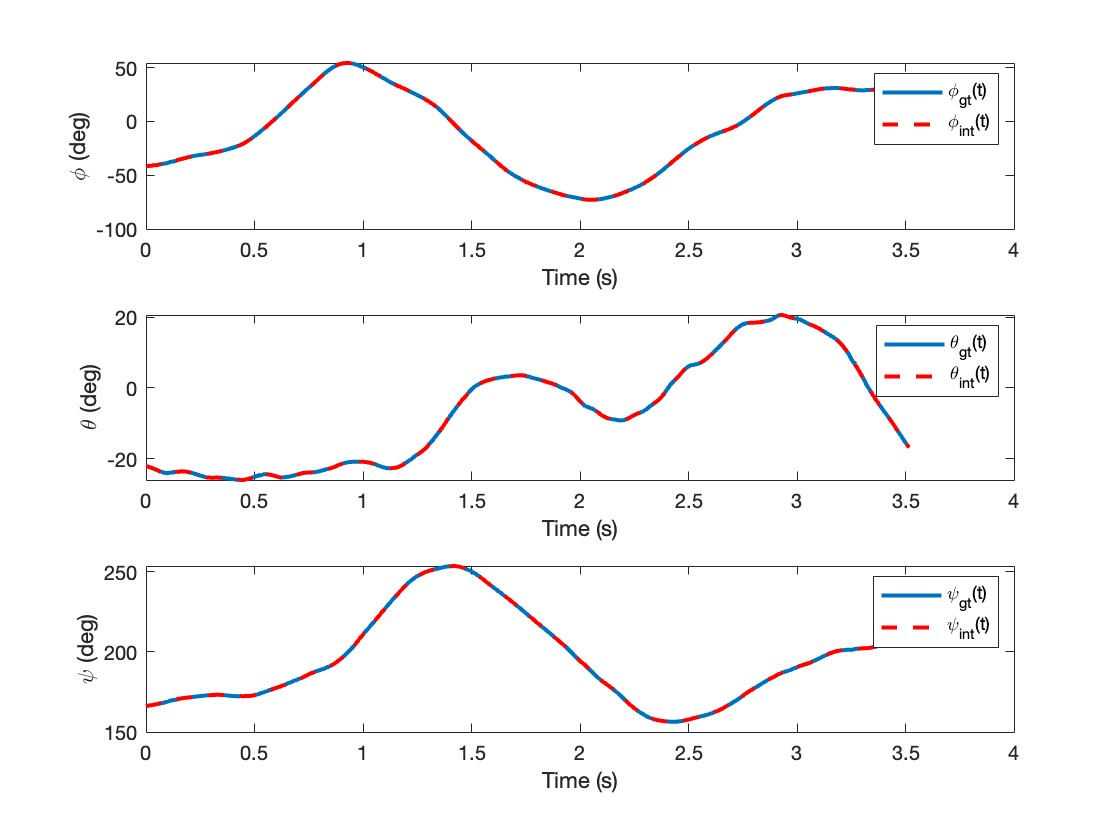
\includegraphics[width=0.8\linewidth]{parta_euler_angles.jpg}
    \caption{Euler Angle Integration vs. Ground Truth}
\end{figure}

\begin{figure}[H]
    \centering
    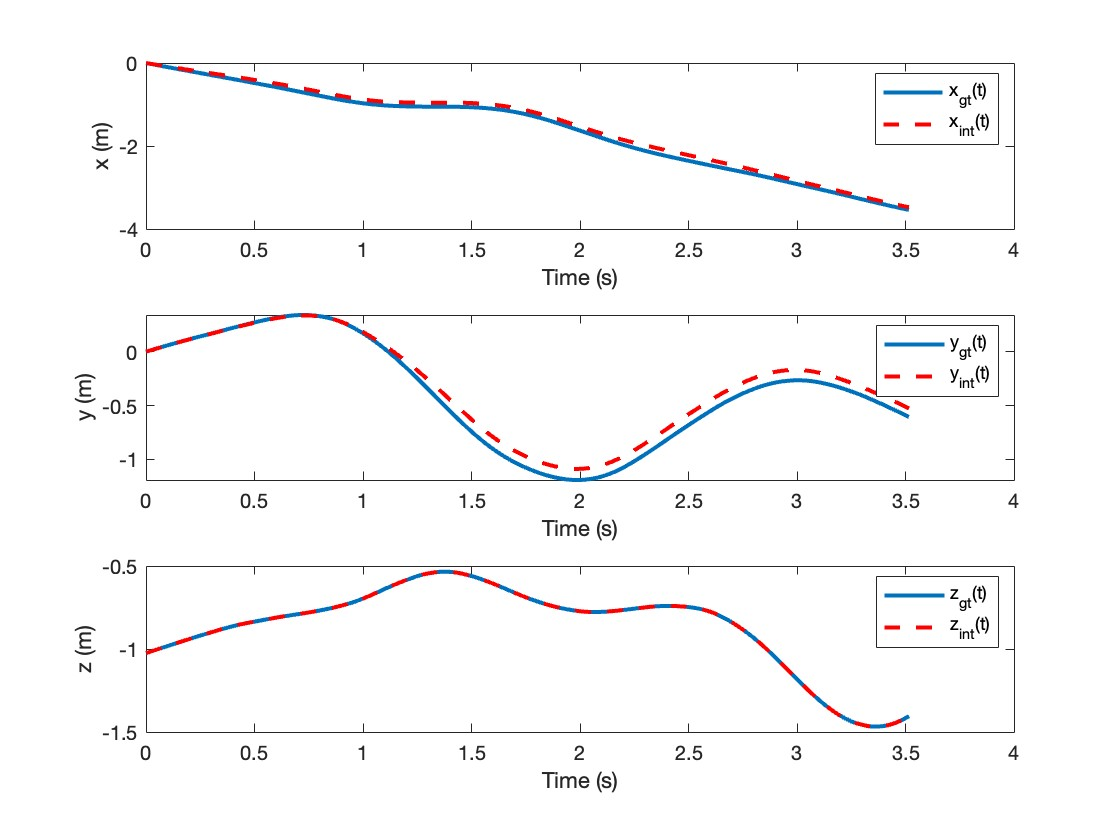
\includegraphics[width=0.8\linewidth]{parta_position.jpg}
    \caption{Position Integration vs. Ground Truth}
\end{figure}

The drift is really an artifact of the integration method chosen. To help rectify this, we can perform an RK4 style integration to better improve the results as shown below.
\lstinputlisting[frame=single, numbers=left, style=Matlab-editor, firstline=1, lastline=86]{hw2_rk4.m}

\begin{verbatim}
    Difference between estimated and ground truth position

error_x =

    0.1738


error_y =

    0.1591


error_z =

    0.0978
\end{verbatim}

We still have some drift but it is less magnified now which is an improvement. Furthermore, other methods like implicit midpoint could also help reduce drift as well. The plot below shows a much better alignment between integration and ground truth positions.
\begin{figure}[H]
    \centering
    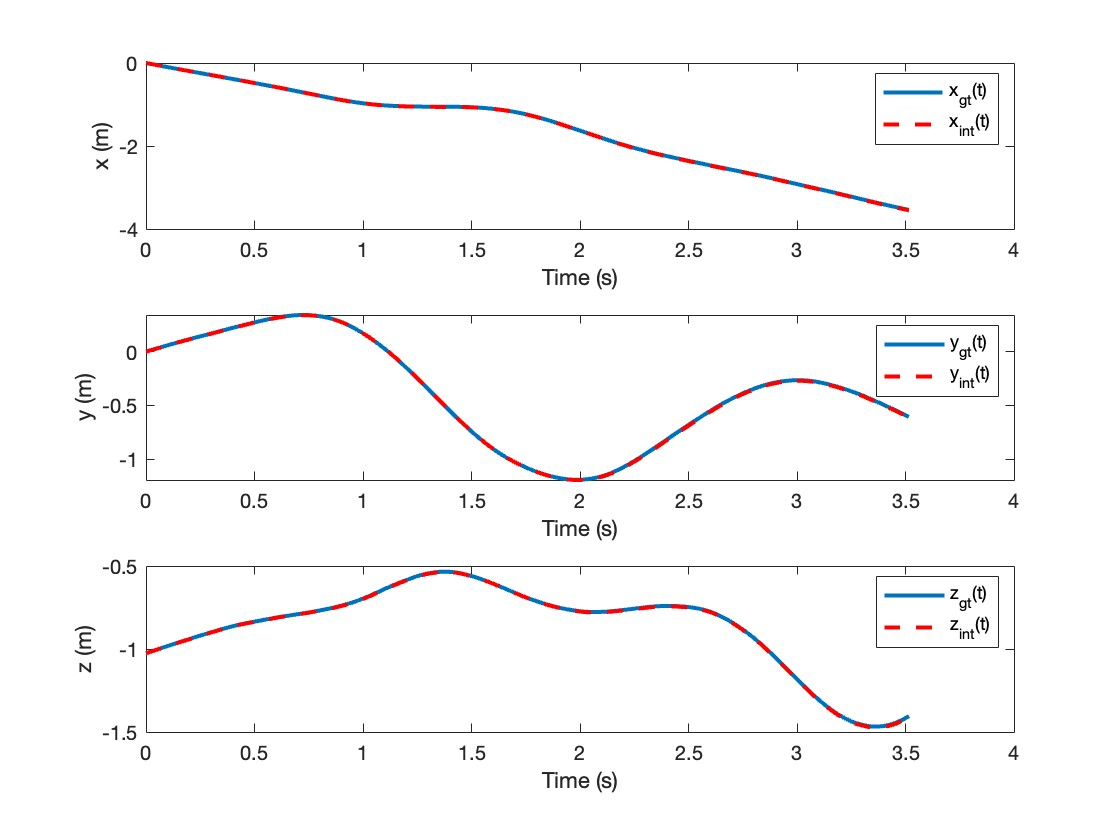
\includegraphics[width=0.8\linewidth]{position_rk4.jpg}
    \caption{Position Integration vs. Ground Truth (RK4)}
\end{figure}

\subsection{Part (b)}

In this part we are asked to perform the same integration except using quaternions now (note the IMU measurements are still the same). The below matlab code snippet shows my approach for this.
\lstinputlisting[frame=single, numbers=left, style=Matlab-editor, firstline=79, lastline=127]{hw2.m}

Note, for this I am using the explicit euler integration so there is still drift but the above RK4 or implicit midpoint integration methods will aid in positional improvements as shown in part (a) above.
\begin{verbatim}
    Difference between estimated and ground truth position

error_x =

    3.8425


error_y =

    3.4988


error_z =

    0.2182
\end{verbatim}

The plotting matlab code for quaternions is shown here:
\lstinputlisting[frame=single, numbers=left, style=Matlab-editor, firstline=1, lastline=43]{plot_quaternion.m}

Below display the resulting plots for the four quaternion values and the position using integration vs. ground truth.

\begin{figure}[H]
    \centering
    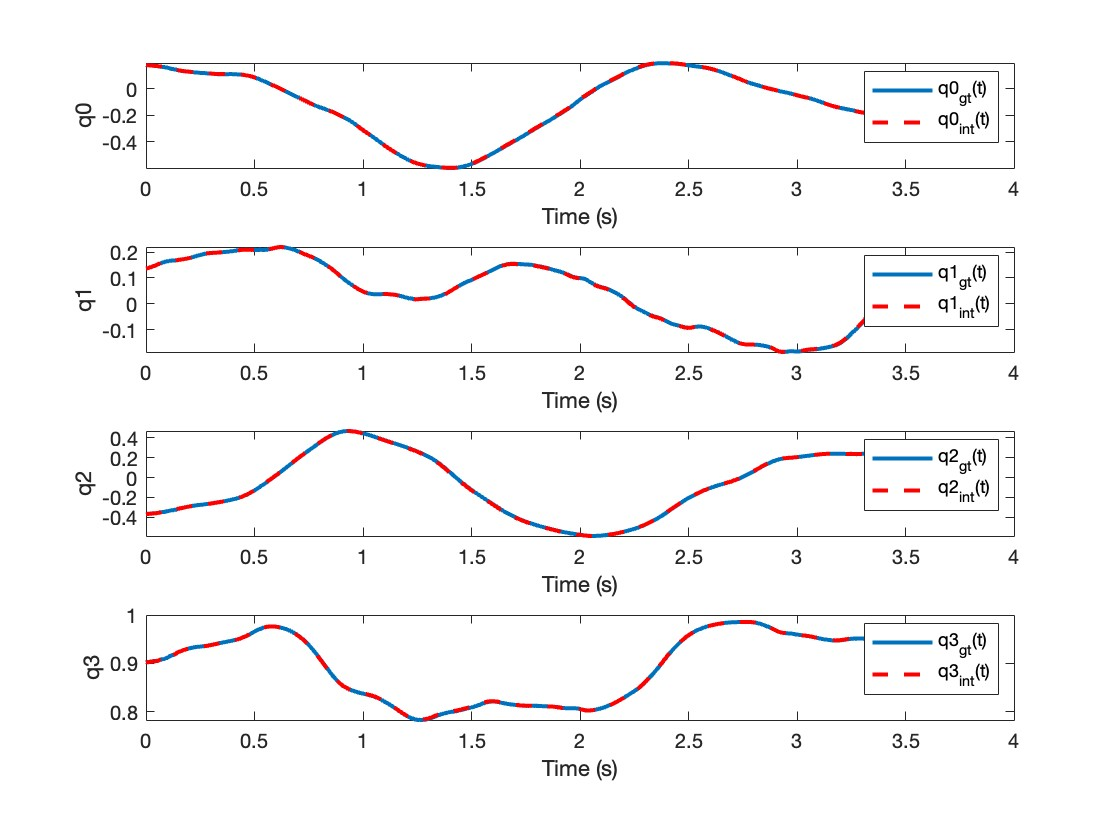
\includegraphics[width=0.8\linewidth]{partb_quaternions.jpg}
    \caption{Quaternion Integration vs. Ground Truth}
\end{figure}

\begin{figure}[H]
    \centering
    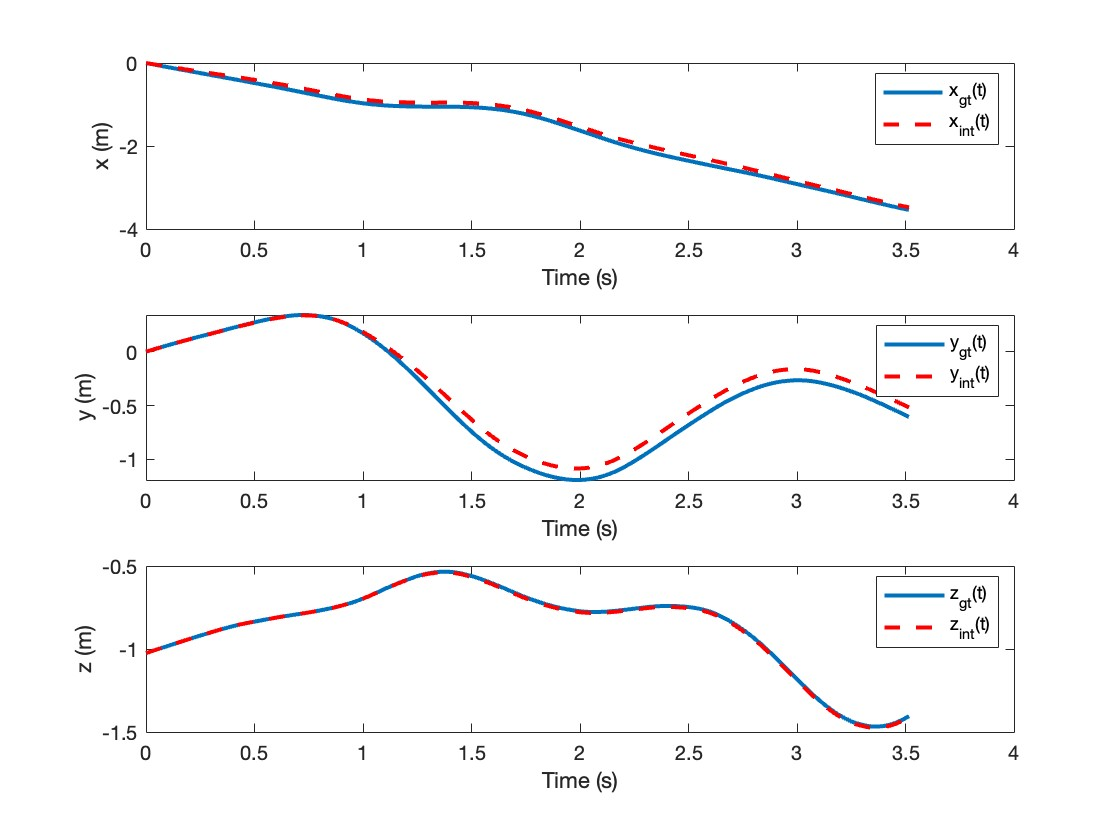
\includegraphics[width=0.8\linewidth]{partb_position.jpg}
    \caption{Position Integration vs. Ground Truth}
\end{figure}

Overall we can visually and quantitativelty see that the integration of euler angles and quaternions are spot on, and quaternions help avoid gimbal lock or singularities, whereas euler angles are susceptible to this phenomena. Likewise, the position can be acquired integrating the velocity components of the IMU measurements but the accuracy is subject to the integration method used. Explicit euler methods will tend to provide worse estimates of position over time vs. RK4 or some other higher fidelity integration scheme as shown in this HW.

\end{document}
